\section{The distributed CA exponential integrator}\label{sec:integrator}

\Cref{sec:gpu} recomputed the opportunity coordinates for a GPU memory system and measured both mechanisms on isolated kernels. The next step is to test a complete solve. This section evaluates a communication-avoiding exponential integrator for the pricing problem in \Cref{sec:model}, distributed over spatial subdomains on up to four V100s across two nodes. The main question is whether the kernel-level savings survive convergence control, the implemented conditioning guard, polynomial boundary forcing, and comparison with an independent semi-discrete referee.

\subsection{The solver}\label{sec:integrator-solver}

The grid is divided into \emph{slabs} along the slowest axis $x_3$, with one slab per GPU. Each device owns a contiguous range of grid planes and the Krylov basis for those rows. This cut makes every off-slab dependency a plane from at most two neighboring devices. Dang, Christara and Jackson divide their single-GPU ADI work into three-dimensional CUDA execution tiles \cite{dang-christara-jackson-2010}. Their tiles organize work inside one device, while the slabs here define ownership between devices. This implementation still uses three-dimensional shared-memory tiles inside each slab. A full three-dimensional multi-GPU decomposition could improve surface-to-volume ratio at larger participant counts, but it would add up to six face neighbors, edge and corner dependencies, and more complicated deep halos. With at most four devices and $O(N_1N_2)$ slow-axis bandwidth, contiguous slabs keep the communication contract manageable.

The required off-slab planes form the \emph{halo}, or ghost region. A device imports this data before applying the operator to its boundary rows. This is where the vertical mechanism reappears at network scale. One stencil application reaches one plane beyond the slab. A matrix-powers Krylov block of width $s$ applies the operator $s-1$ times and reaches $s-1$ planes out. One \emph{deep} exchange of those planes replaces $s-1$ shallow exchanges. The number of bytes remains the same, as \Cref{sec:integrator-depth} confirms, but the message count falls from $s-1$ to one. That reduction matters on a latency-dominated fabric.

The remaining solver follows \Cref{sec:ksm-ca}. It applies the operator \emph{matrix-free}, computing the 19-point stencil directly instead of storing and multiplying an assembled sparse matrix. This removes matrix-index traffic. A CUDA thread block stages an interior tile and its ghost layers in shared memory, then runs the recurrence. CholeskyQR2 orthogonalizes each Krylov block. The device evaluates the operational guard $\kappa_2(\mat{Z})\le u^{-1/2}$ and narrows any block that exceeds it. As discussed in \Cref{sec:ksm-ca}, this policy targets practical normal-equations breakdown; the dimension-dependent sufficient condition and distributed Gram rounding are assessed separately \cite{yamamoto-2015,fukaya-2014}. Local Krylov-block Gram matrices and projections are combined with NCCL all-reduces, while halos use NCCL send/receive pairs \cite{yamazaki-2014}. Since $m\le39$, the projected $\mat{H}_m$ is at most $39\times39$, and every device can replicate the small exponential.

Correctness is checked with an instrument that shares no stencil code with the production path. The referee assembles the $N+3$ Basket operator $\widetilde{\mat{A}}$, or the unaugmented Rainbow operator, as a sparse matrix. It applies the matrix with the vendor library and evaluates the exponential action with the Al-Mohy--Higham Taylor method \cite{almohy-higham-2011}. Reported arms pass the convergence and conditioning guards, preserve the forcing tail or Rainbow boundary state, and agree with an arm-matched single-GPU result and the independent semi-discrete reference within the stated tolerances. These checks provide direct evidence for the tested numerical path. Theorem-level CholeskyQR2 coverage and the total financial-error budget remain separate questions.

Device contention is checked before timing because a competing process can consume memory bandwidth, cache capacity, and streaming multiprocessors. Slurm reserves the requested Synge nodes, and NVML provides an additional idle-device gate. Adaptive decisions are compared across ranks before each collective, so disagreement aborts instead of deadlocking.

\subsection{Recurrence depth, and what a fair control costs}\label{sec:integrator-depth}

A Krylov block of width $s$ contains $[\vect v,\mat A\vect v,\ldots,\mat A^{s-1}\vect v]$. It requires exactly $s-1$ recurrence applications and a deep halo $s-1$ planes wide. Every reported performance result follows this exact-depth rule. The rule makes $s=1$ a fair non-CA control: one ordinary Arnoldi operator application and one halo plane per basis vector, with no unused power.

\begin{table}[htbp!]
\centering
\caption{Halo planes moved per Krylov basis vector under the exact-depth rule, $n=97$ on four V100s. The measured column comes from the solver's exchange-depth histogram.}
\label{tab:ca-depth}
\begin{tabular}{@{}llrrr@{}}
\toprule
\textbf{Rule} & $s$ & \textbf{Exchanges/time step} & \textbf{Planes per vector} & \textbf{Predicted} \\
\midrule
\texttt{exact-depth} & 1 & 11.45--11.48 & 1.000 & 1 \\
\texttt{exact-depth} & 4 & 6.40--6.46  & 1.000 & 1 \\
\bottomrule
\end{tabular}
\end{table}


Both widths move one halo plane per basis vector, so $s$-step reduces message count rather than message volume. The $s=4$ Krylov block contains four planes of powers, from degree 0 through degree 3, and therefore needs three operator applications; each application extends the stencil radius by one plane, giving a three-plane deep halo. Across the two payoffs its 5{,}645--5{,}698\,KiB per time step exceeds the $s=1$ arm's 5{,}050--5{,}063\,KiB because a fixed depth-one transition exchange is amortized over four vectors.

\subsection{Strong scaling}\label{sec:integrator-strong}

Strong scaling asks whether additional devices reduce latency at fixed global work. The control uses $n=61$ (226{,}981 unknowns), 100 time steps, tolerance $10^{-8}$, $m_{\max}=39$, a monomial basis, and CholeskyQR2. Every value is a seven-repeat median on idle devices that pass the NVML gate (\Cref{tab:ca-strong}, \Cref{fig:ca-strong}).

\begin{table}[htbp!]
\centering
\caption{Exact-depth strong scaling at $n=61$, showing cycle time in ms/time step, seven-repeat medians, and CA speedup $t(s{=}1)/t(s{=}4)$.}
\label{tab:ca-strong}
\begin{tabular}{@{}lrrcrrc@{}}
\toprule
& \multicolumn{3}{c}{\textbf{Basket}} & \multicolumn{3}{c}{\textbf{Rainbow}} \\
\cmidrule(lr){2-4}\cmidrule(lr){5-7}
\textbf{Topology} & $s{=}1$ & $s{=}4$ & \textbf{CA} & $s{=}1$ & $s{=}4$ & \textbf{CA} \\
\midrule
One V100                & 2.170 & 2.214 & \textbf{0.98$\times$} & 2.187 & 2.172 & \textbf{1.01$\times$} \\
Two V100s, one node     & 3.006 & 2.221 & 1.35$\times$ & 2.985 & 2.197 & 1.36$\times$ \\
Two V100s, two nodes    & 3.864 & 2.845 & 1.36$\times$ & 3.864 & 2.798 & 1.38$\times$ \\
Four V100s, two nodes   & 4.434 & 2.484 & \textbf{1.78$\times$} & 4.389 & 2.433 & \textbf{1.80$\times$} \\
\bottomrule
\end{tabular}
\end{table}

The exact-depth arms are at parity on one GPU. Relative to $s=1$, $s=4$ is $0.98\times$ as fast for Basket and $1.01\times$ for Rainbow. One GPU has no inter-device collectives or halo exchanges to avoid, so the wider Krylov block gives no material end-to-end advantage in this local-work control. At four GPUs, participant count also changes occupancy, launch behavior, and subdomain size, so communication cannot be assigned as the only cause of every difference.

The distributed advantage depends on topology. Across the measured configurations, the CA ratios are $0.98$, $1.35$, $1.36$, and $1.78\times$ for Basket, and $1.01$, $1.36$, $1.38$, and $1.80\times$ for Rainbow. The four rungs increase monotonically, but they do not establish a participant-count scaling law or justify extrapolation beyond the tested systems. Under exact depth, the $s=4$ shared tile holds 1{,}400 doubles per 128 interior points. \Cref{sec:integrator-vertical} measures sensitivity to this geometry directly.

\begin{figure}[t!]
\centering
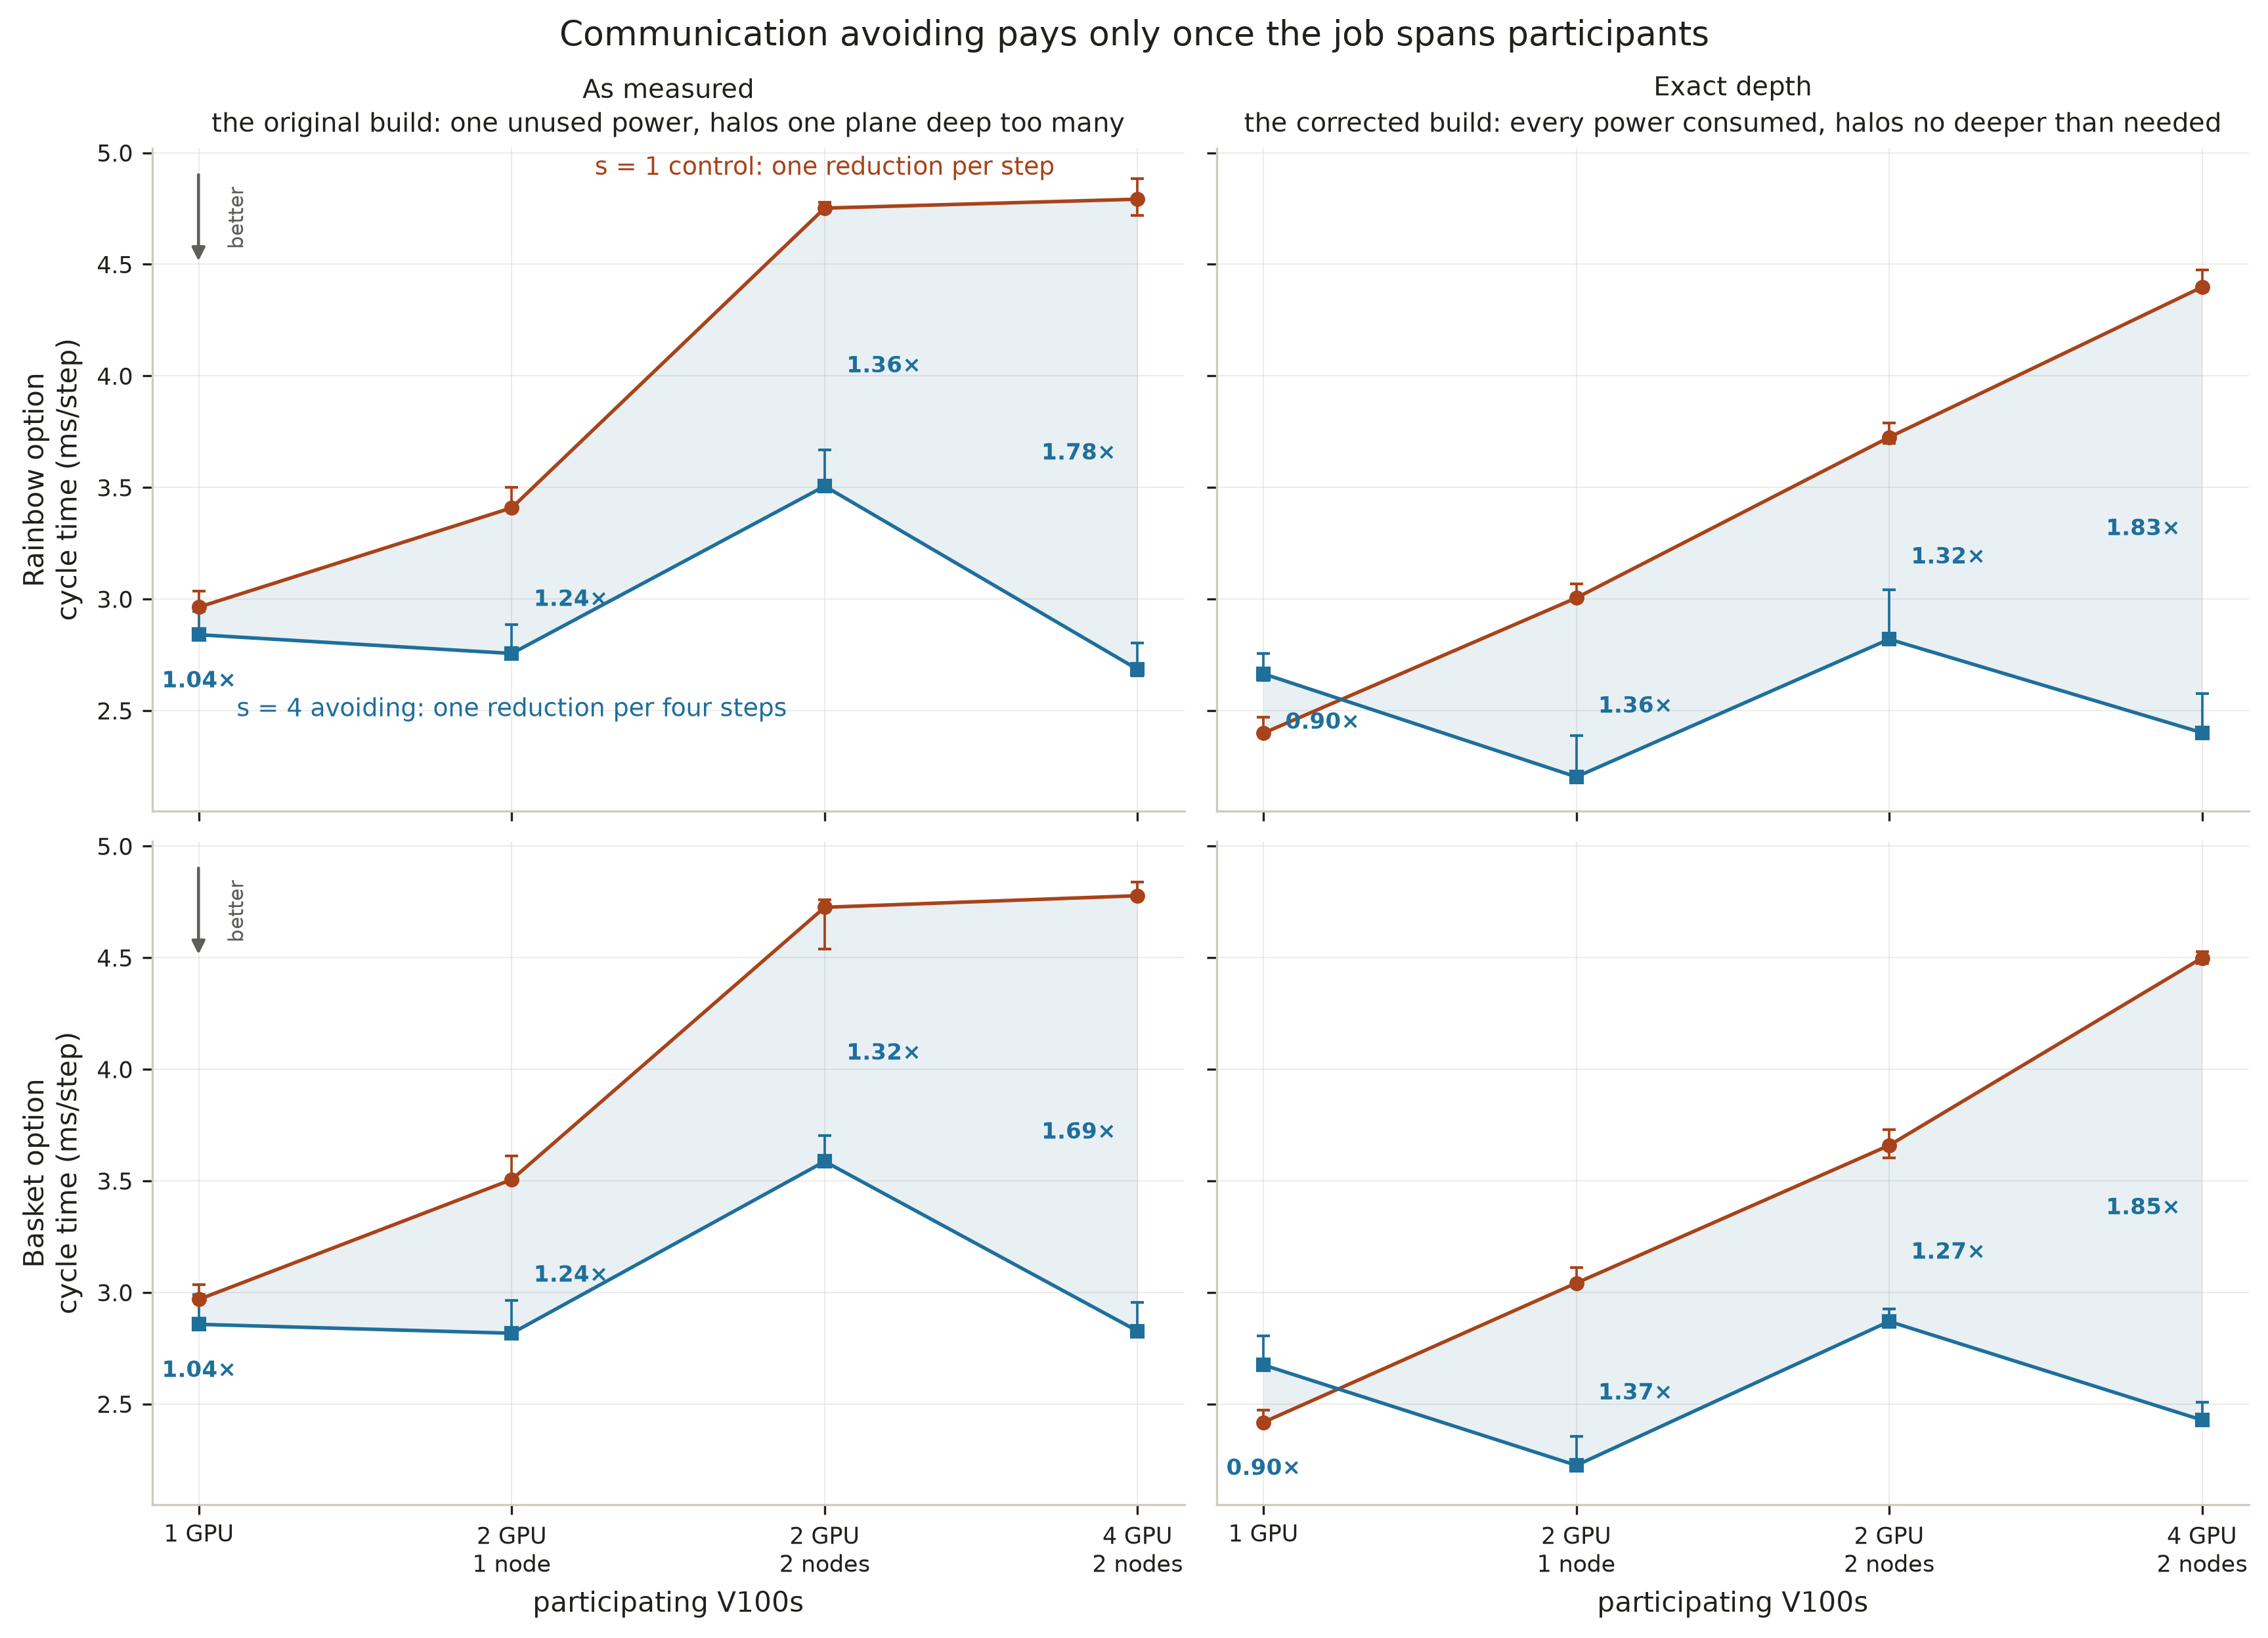
\includegraphics[width=0.68\textwidth]{ca_strong_scaling.png}
\caption{Strong scaling at $n=61$ on Synge V100s for both payoffs and both recurrence-depth controls. Marks are seven-repeat medians with the observed range. For the final exact-depth arm, the single-GPU CA ratio is near one and the four-GPU ratio is 1.78--1.80.}
\label{fig:ca-strong}
\end{figure}

Absolute scaling at this size is poor. Four V100s at $s=4$ deliver only $0.89\times$ the one-V100 performance at the same width. Strong-scaling efficiency is speedup divided by participant count, giving $0.89/4\approx0.22$, or about 22\%. The best four-GPU time is 12--15\% slower than the best one-GPU time across the two payoffs. At $n=61$, each of the four slabs owns roughly 57{,}000 rows, which is too little work to saturate a V100.

The two ratios answer different questions. The algorithm-relative result is 1.78--1.80$\times$ and asks whether $s=4$ beats $s=1$ on the same four-GPU topology. The $0.89\times$ same-width result asks whether four GPUs running $s=4$ beat one GPU running $s=4$. Communication avoidance helps at the measured distributed point, but distributing this small complete solve is still counterproductive.

\subsection{The communication account}\label{sec:integrator-account}

To interpret the difference without fitting the solver, the cost model uses independent microbenchmarks containing only communication. Bare all-reduces and halo exchanges are timed at the integrator's payloads on idle devices for each participant count (\Cref{tab:ca-participants}).

\begin{table}[htbp!]
\centering
\caption{Participant calibration on idle Synge V100s across two nodes, showing the seven-repeat median latency of a bare NCCL all-reduce at the payloads the solver uses. Doubling the participant count is a real cost that a single node-tier constant cannot express.}
\label{tab:ca-participants}
\begin{tabular}{@{}lrrrc@{}}
\toprule
\textbf{Operation} & \textbf{Payload} & \textbf{2 participants} & \textbf{4 participants} & \textbf{Ratio} \\
\midrule
Norm                & 8\,B    & 20.06\,$\mu$s & 29.20\,$\mu$s & 1.46$\times$ \\
Gram, $s{=}1$       & 8\,B    & 20.94\,$\mu$s & 28.26\,$\mu$s & 1.35$\times$ \\
Projection, $s{=}1$ & 200\,B  & 22.32\,$\mu$s & 31.35\,$\mu$s & 1.40$\times$ \\
Gram, $s{=}4$       & 128\,B  & 21.91\,$\mu$s & 31.16\,$\mu$s & 1.42$\times$ \\
Projection, $s{=}4$ & 800\,B  & 23.32\,$\mu$s & 38.31\,$\mu$s & 1.64$\times$ \\
64\,MiB all-reduce  & 64\,MiB & 9.51\,ms      & 12.51\,ms     & 1.32$\times$ \\
\bottomrule
\end{tabular}
\end{table}

Adding participants increases latency because an all-reduce must combine more contributions and traverse more links or tree/ring stages. Completion also waits for the slowest participant. On Synge, moving from two to four participants can cross both PCIe/socket and inter-node boundaries. The 8-byte rows show that cost grows even when the payload does not.

The solver transcript counts every collective and halo exchange. Each operation is priced with its calibrated latency, using the depth actually exchanged by that arm, and subtracted from the measured cycle. The remainder is local work, so no solver-time coefficient is fitted (\Cref{fig:ca-decomposition}). In the final correction sweep, this account assigns 31--36\% of the $s=1$ cycle and 11--20\% of the $s=4$ cycle to communication. Participant count and payload explain much of the algorithm-relative difference. The non-additivity check below prevents the decomposition from being treated as a causal proof.

\begin{figure}[t!]
\centering
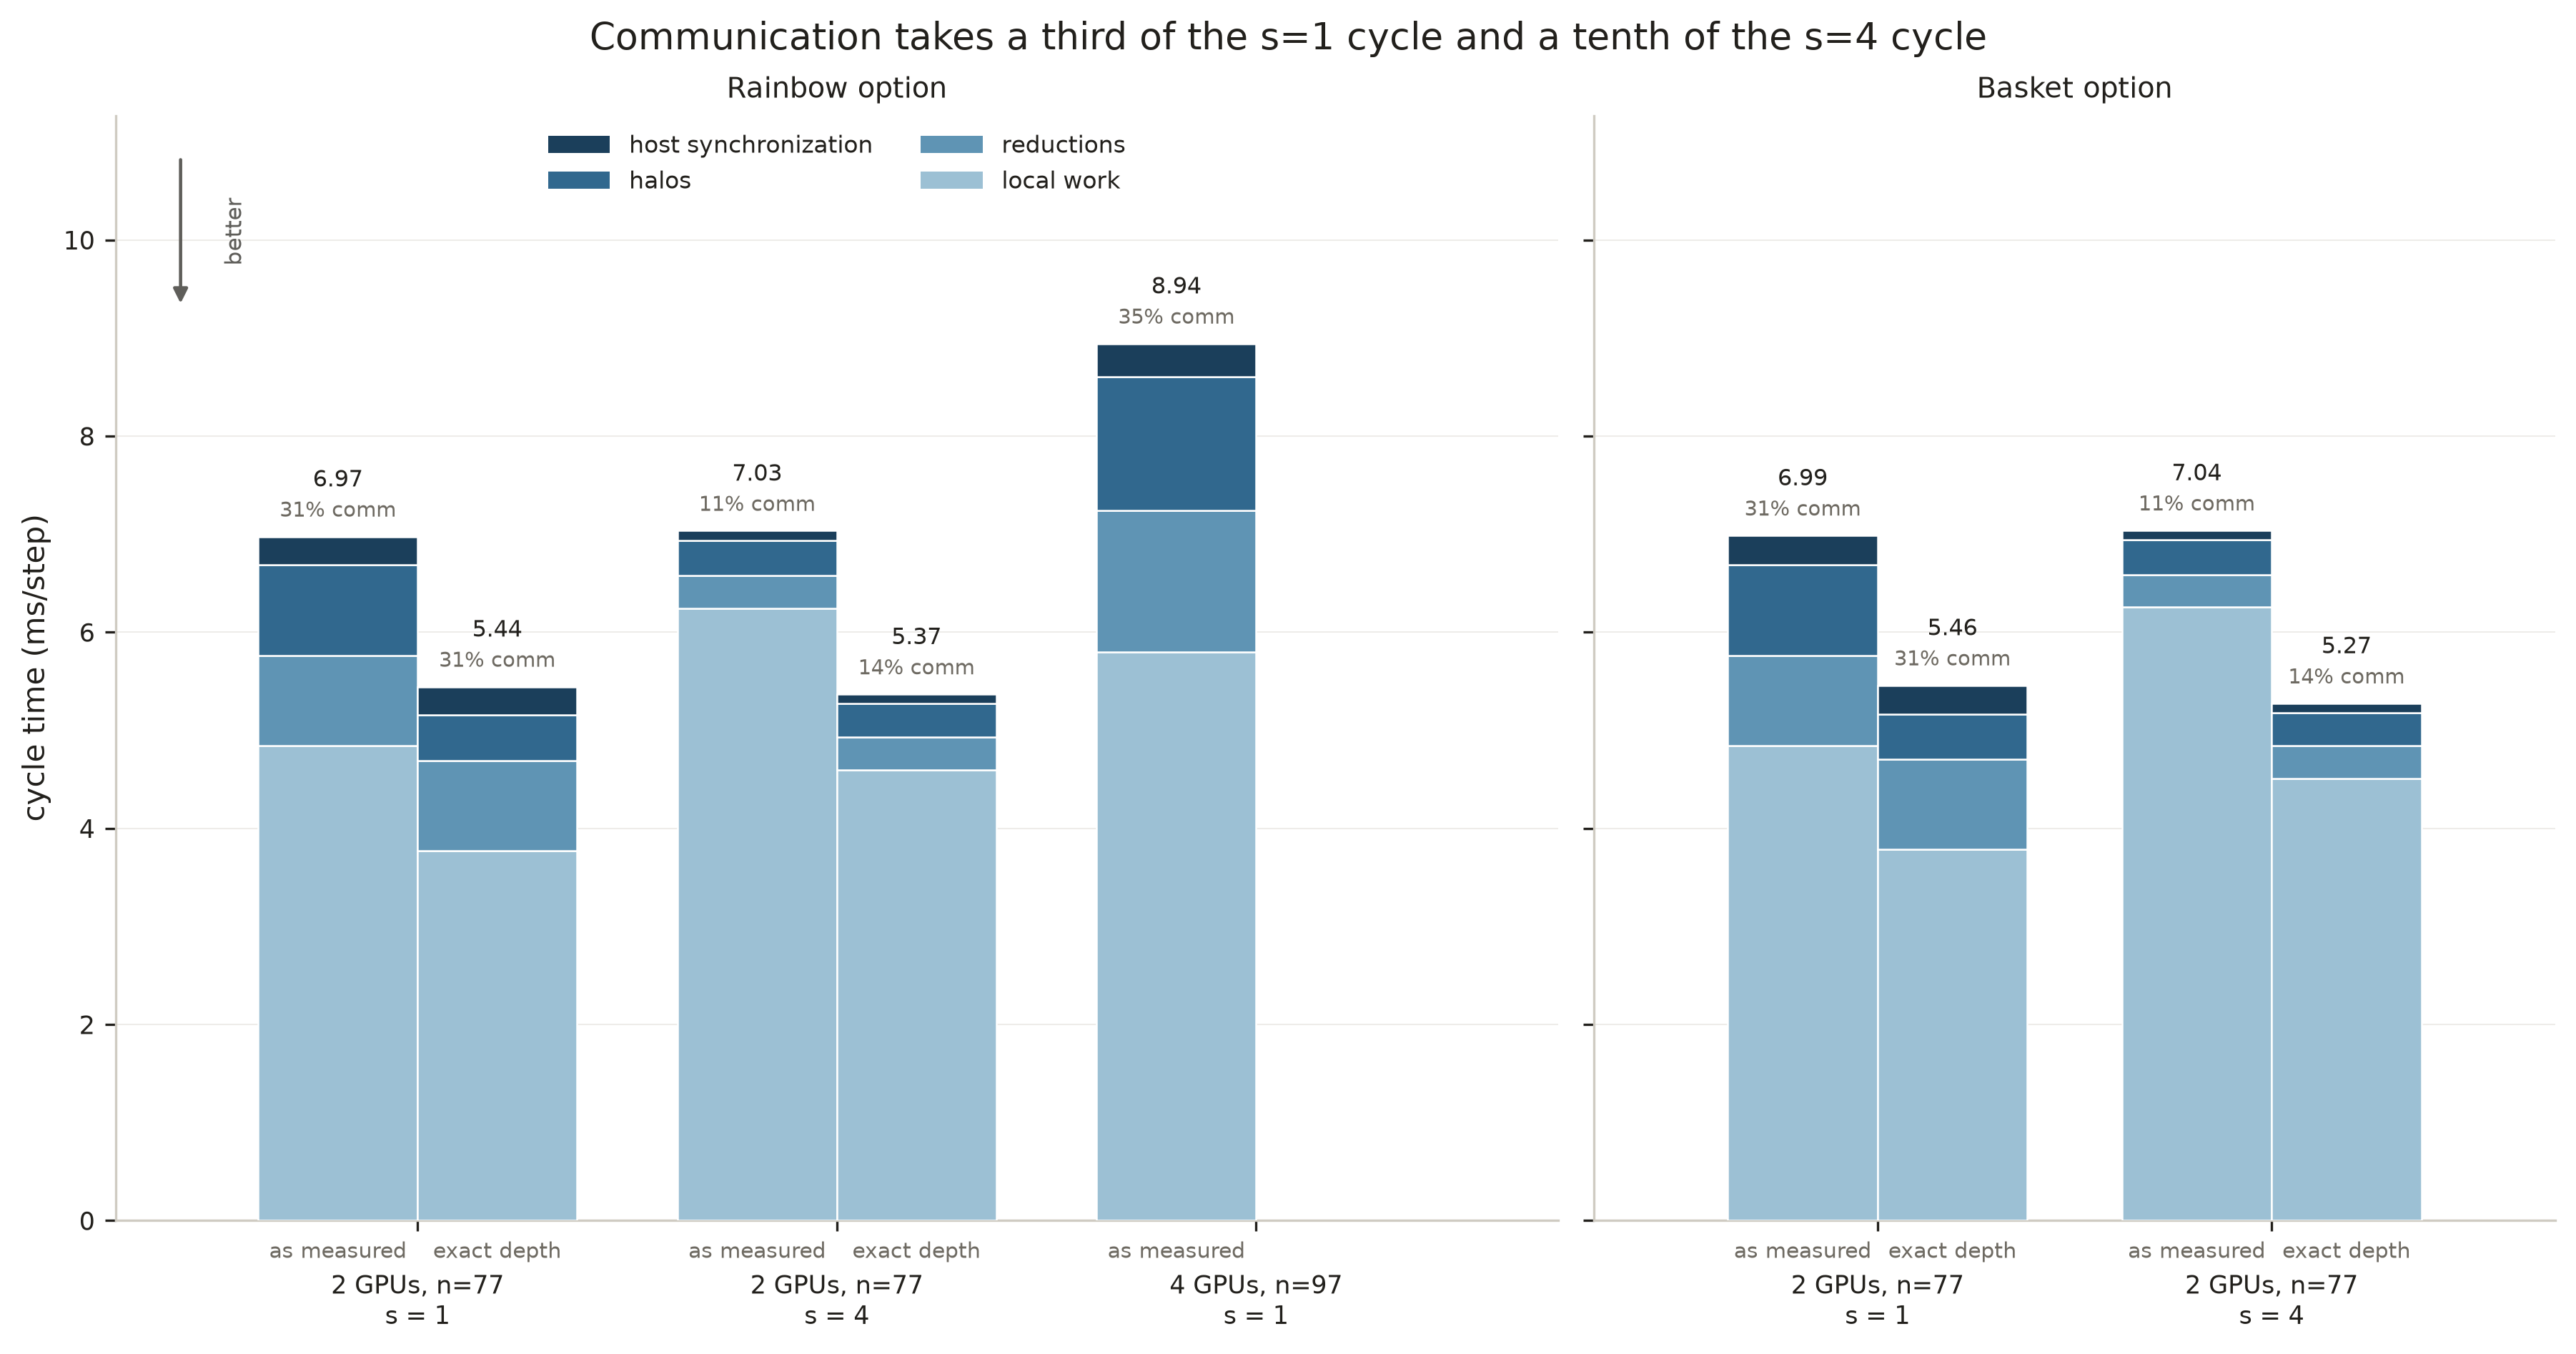
\includegraphics[width=0.82\textwidth]{ca_cycle_decomposition.png}
\caption{Cycle-time decomposition on Synge V100s across two nodes. Reductions and halos are transcript counts priced by the participant calibration; local work is the remainder, so no term is fitted. Bars carry the total cycle time and the share of it spent communicating.}
\label{fig:ca-decomposition}
\end{figure}

Agreement is close but not exact because communication costs are not additive. Summing reductions, deep exchanges, and host round-trips over-counts work that overlaps on the device. For example, the conditioning diagnostic returns to the host before deciding whether to narrow the Krylov block. At $n=61$ on four GPUs, the corrected $s=1$ arm performs 35.1 round-trips per time step and stalls for 2.02\,ms; the $s=4$ arm performs 10.7 and stalls for 1.66\,ms. Each host wait also drains queued device work. The measured stall is therefore an upper bound on recoverable overhead and is not added to the communication account.

Non-additivity suggests that halo transfers could be hidden behind independent interior work, a standard CUDA stream optimization. An explicit experiment compares serialized exchange with copy--compute overlap on two V100s in one node at $n=61$, $s=3$. The overlapped states pass the $10^{-12}$ agreement gate. An Nsight Systems trace shows that 99.7\% of peer-halo copy time overlaps matrix powers, compared with 0\% in the serialized arm. Even so, wall-clock time does not improve. The seven-repeat median changes from 2.323 to 2.379\,ms per time step for Basket and from 2.304 to 2.329\,ms for Rainbow, with overlapping ranges. Splitting one slab launch into an interior launch and two boundary launches triples the profiled launch count. That overhead offsets the hidden copy time, so serialized exchange remains the default.

\subsection{The vertical coordinate, measured}\label{sec:integrator-vertical}

The CPU study could not count DRAM traffic, and its tiled kernel never became bandwidth-bound (\Cref{sec:vertical}). On the GPU, privilege-free counters compare measured DRAM traffic with modeled demand at 44 idle-device points covering four widths, four grids, both payoffs, and four tile geometries (\Cref{tab:ca-vertical}, \Cref{fig:ca-roofline}).

A spatial tile is the three-dimensional interior region assigned to one CUDA thread block: $8\times4\times4$, for example, covers 8 points in $x_1$, 4 in $x_2$, and 4 planes in $x_3$ before adding $s$-dependent shared-memory ghosts. Larger tiles reduce redundant ghost reads but may lower occupancy or access efficiency.

\begin{table}[htbp!]
\centering
\caption{The matrix-powers kernel against both roofs at $n = 97$ (Rainbow, full-volume $8\times4\times4$ baseline, idle V100, counter-measured DRAM traffic). Redundancy is the ratio of shared-tile reads to distinct interior points. No width comes within reach of either roof.}
\label{tab:ca-vertical}
\begin{tabular}{@{}rrrrl@{}}
\toprule
$s$ & \textbf{Ghost redundancy} & \textbf{DRAM roof} & \textbf{L2 roof} & \textbf{Verdict} \\
\midrule
1 & 2.81$\times$  & 54.9\% & 3.8\% & latency-bound \\
2 & 6.00$\times$  & 21.1\% & 2.3\% & latency-bound \\
3 & 10.94$\times$ & 8.0\%  & 1.6\% & latency-bound \\
4 & 18.00$\times$ & 2.1\%  & 1.2\% & latency-bound \\
\bottomrule
\end{tabular}
\end{table}

\begin{figure}[t!]
\centering
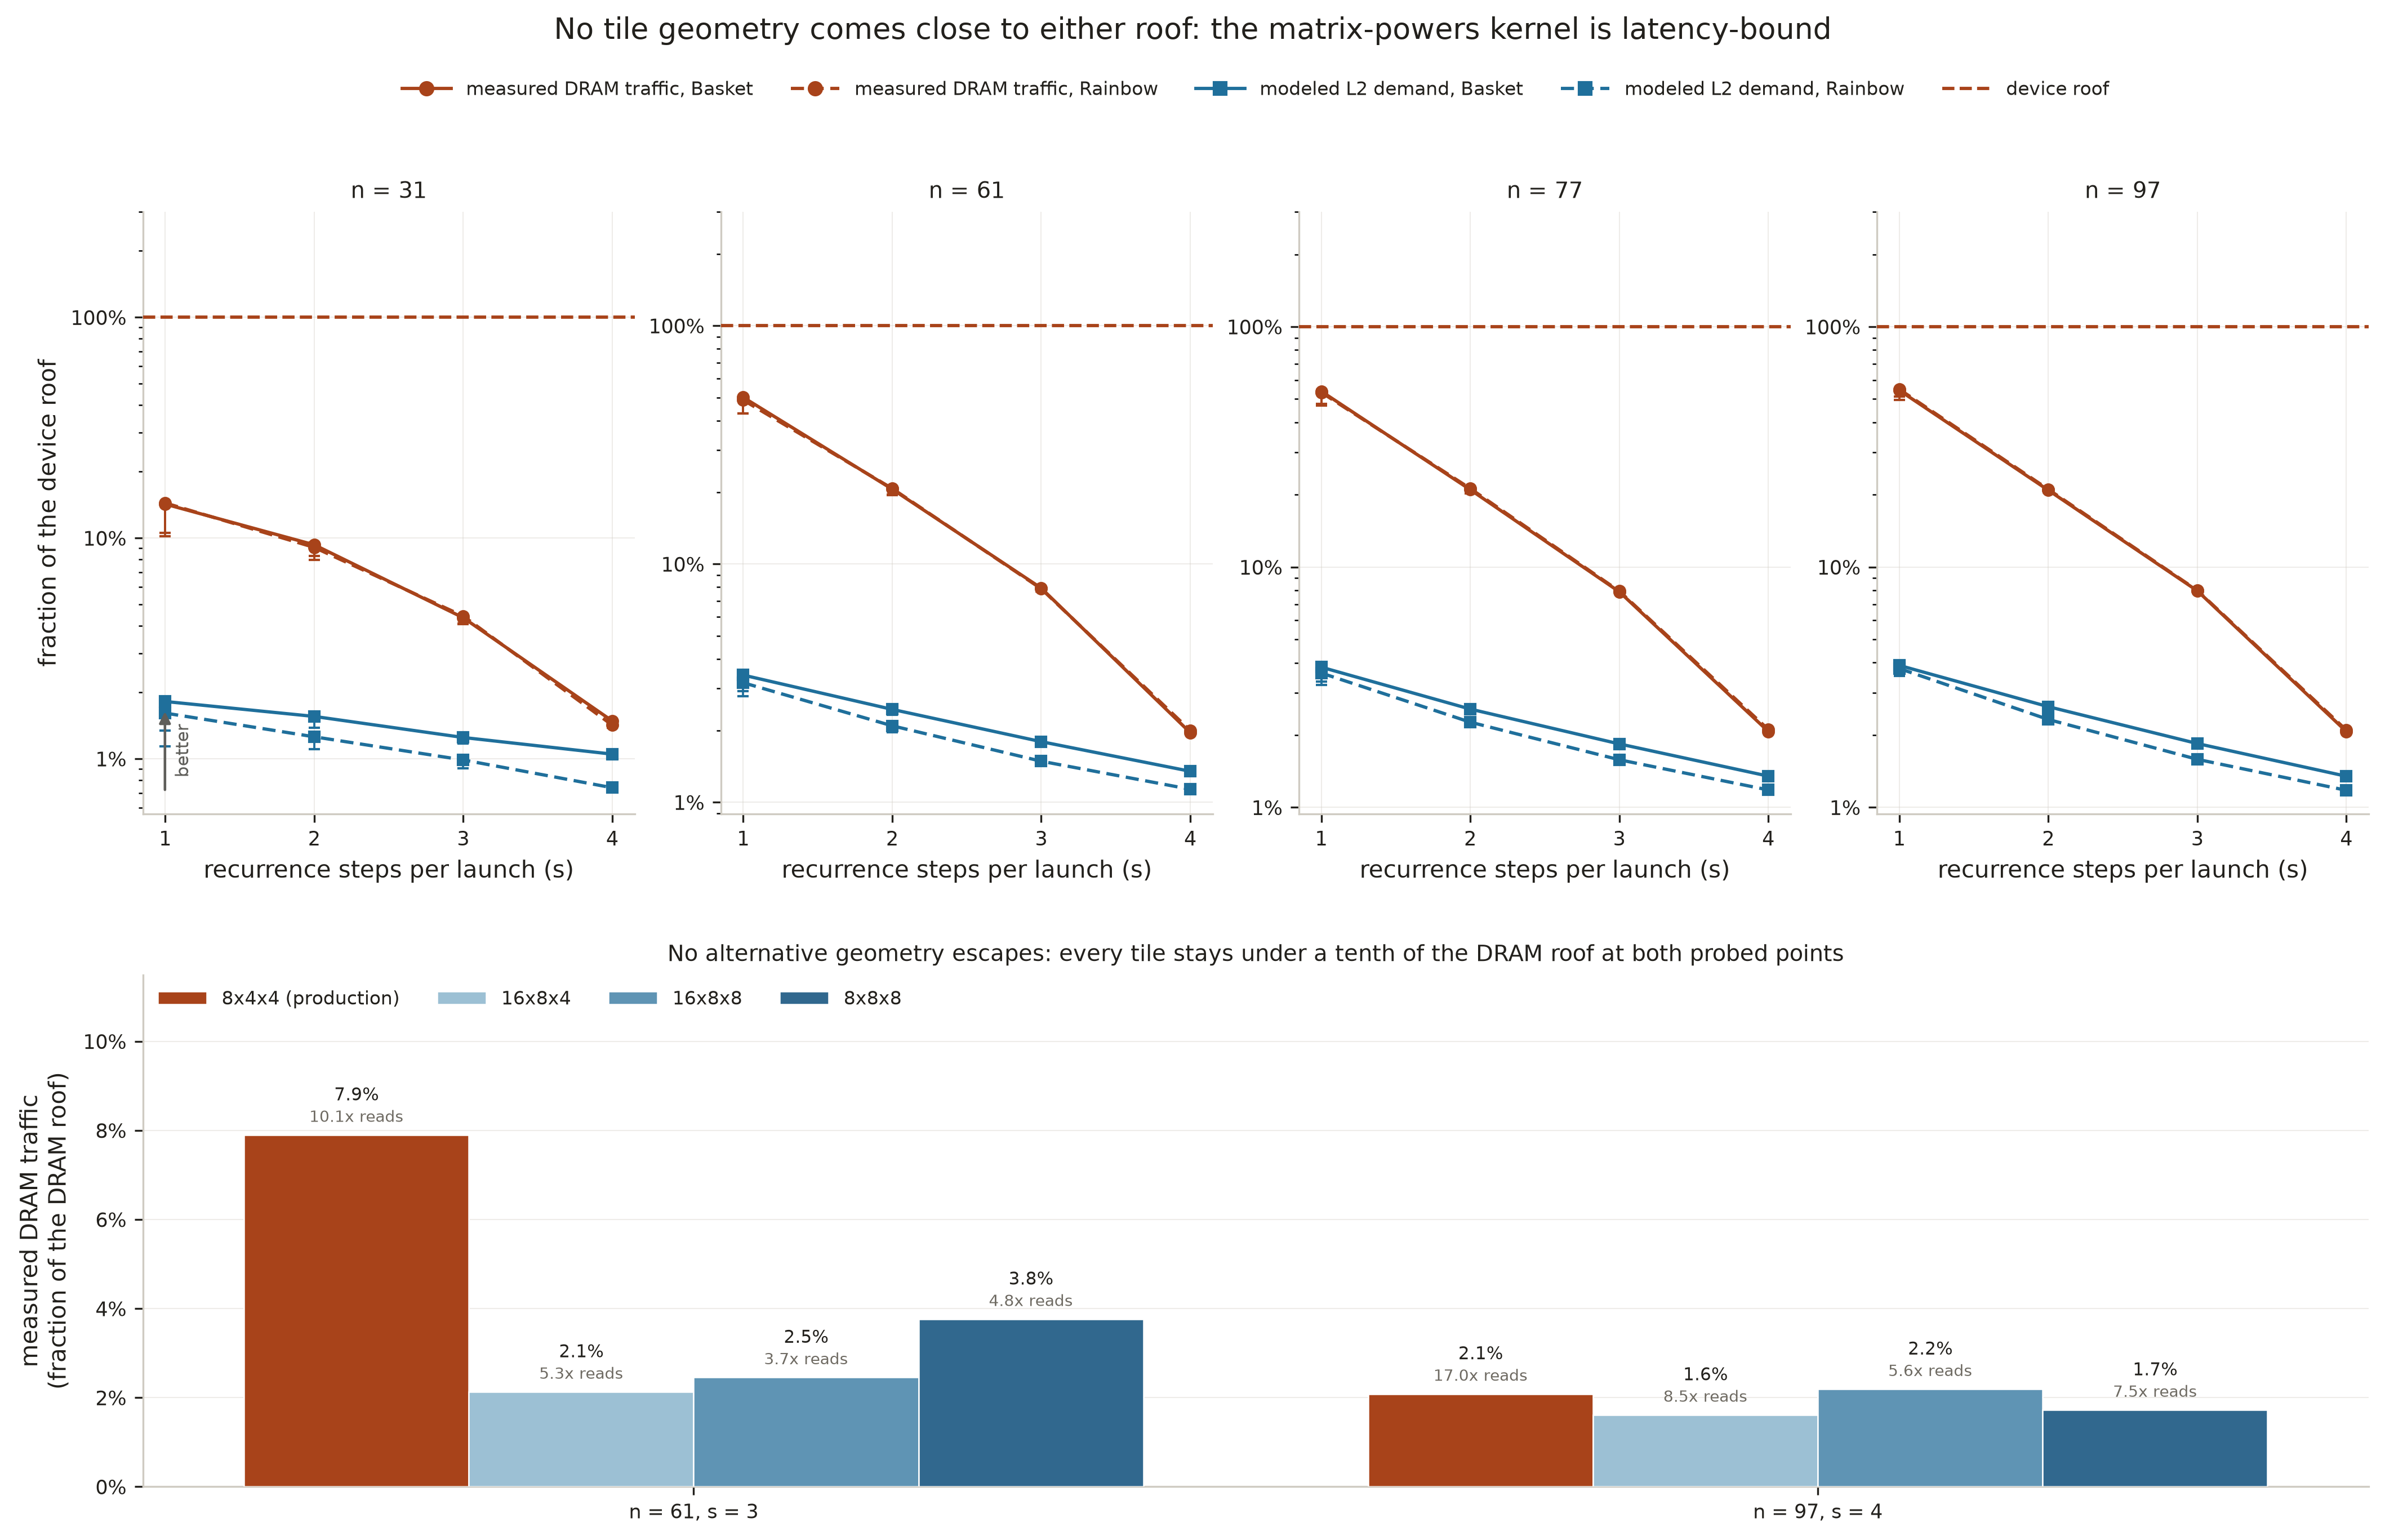
\includegraphics[width=0.8\textwidth]{ca_matrix_powers_roofline.png}
\caption{Matrix-powers traffic relative to the V100 device roofs (seven-repeat medians). Top: measured DRAM traffic and modeled L2 demand across widths and grids. Bottom: measured DRAM traffic for four geometries at the two tuning points; annotations give effective read redundancy.}
\label{fig:ca-roofline}
\end{figure}

The classifier separates traffic location from the kernel limiter. An earlier rule labeled a width \emph{L2-absorbed} when measured DRAM traffic fell well below modeled tiled demand. However, a kernel reaching only 1.2\% of the L2 roof is not L2-bound. Traffic attribution is therefore reported separately through the measured-to-modeled byte ratio: 3.3, 2.0, 1.1, and 0.40 as $s$ increases from 1 to 4. The model under-counts narrow tiles because one tile row straddles several memory sectors. It over-counts wide tiles because overlap between neighboring spatial tiles remains in L2.

Roof-based attribution classifies all 44 points as \emph{latency-bound}. The largest DRAM fraction is 0.55 against a 0.75 threshold, and the largest L2 fraction is 0.04. Nsight defines \emph{Wait} as a warp stalled on a fixed-latency execution dependency and \emph{Long Scoreboard} as a warp waiting for an L1TEX result from local, global, surface, or texture memory \cite{nvidia-nsight-compute}. Wait dominates 15 of 16 scheduler captures. Long Scoreboard leads only for Rainbow on the full-volume baseline at $n=61$, $s=3$. Occupancy is not treated as the limiter because lower-occupancy configurations sometimes run faster in this controlled sweep.

The $8\times8\times8$ and $16\times8\times8$ configurations test progressively larger volumes, while $16\times8\times4$ keeps the same 512-point interior volume as $8\times8\times8$ with a different aspect ratio. \Cref{tab:ca-tiles} separates volume from shape at the two canonical points.

\begin{table}[htbp!]
\centering
\caption{Tile geometry sweep on an idle V100, seven-repeat medians. Redundancy is the effective in-domain read redundancy; speedup is against the full-volume $8\times4\times4$ baseline at the same point, given as the range over the two payoffs. Occupancy is quoted for $(n{=}61, s{=}3)$ and $(n{=}97, s{=}4)$ respectively.}
\label{tab:ca-tiles}
\begin{tabular}{@{}lcrcrc@{}}
\toprule
& & \multicolumn{2}{c}{$n = 61$, $s = 3$} & \multicolumn{2}{c}{$n = 97$, $s = 4$} \\
\cmidrule(lr){3-4}\cmidrule(lr){5-6}
\textbf{Tile} & \textbf{Occupancy} & \textbf{Redund.} & \textbf{Speedup} & \textbf{Redund.} & \textbf{Speedup} \\
\midrule
$8\times4\times4$ (baseline) & 0.250 / 0.125 & 10.07$\times$ & 1.00$\times$ & 17.03$\times$ & 1.00$\times$ \\
$8\times8\times8$   & 0.125 / 0.0625 & 4.81$\times$ & \textbf{1.33--1.39$\times$} & 7.52$\times$ & 0.96--1.02$\times$ \\
$16\times8\times8$  & 0.0625 & 3.69$\times$ & 1.10--1.21$\times$ & 5.62$\times$ & \textbf{1.28--1.36$\times$} \\
$16\times8\times4$  & 0.0625 & 5.34$\times$ & 0.95--1.04$\times$ & 8.45$\times$ & 0.98--1.04$\times$ \\
\bottomrule
\end{tabular}
\end{table}

Neither candidate limiter explains the fixed-geometry sweep alone. The winning geometry has \emph{lower} occupancy than the baseline in every case; quartering occupancy makes the kernel faster. Ghost redundancy is also insufficient by itself. At $n=61$, the lowest-redundancy tile ($16\times8\times8$) moves the least traffic but still loses to $8\times8\times8$. At $n=97$, the lowest-traffic tile is 30\% slower than the winner. A wider tile removes redundant bytes but can reduce access efficiency, and the balance changes with the grid.
No single full-volume shape won across all tested points. Selecting the best geometry separately for each grid gives only $1.08\times$ solver speedup at $s=1$ and $1.13\times$ at $s=4$, despite a $1.33$--$1.39\times$ gain for the isolated kernel, and the winning shape changes with $(n,s)$.

The follow-on design changes the schedule instead of choosing another fixed three-dimensional tile. A CUDA thread block owns a $16\times8$ tile in the $x$--$y$ plane and walks a contiguous $z$ segment. It keeps a circular queue of planes for each recurrence level. Because the shared-memory footprint is independent of segment height, a longer segment amortizes the $z$ prologue and epilogue without enlarging the resident queue. The predeclared automatic rule keeps the full-volume baseline below $n=61$. At larger grids, it selects the segment height closest to eight $z$-directed CUDA thread blocks, subject to the device's opt-in shared-memory limit. An inadmissible recurrence width falls back instead of failing.

\begin{table}[htbp!]
\centering
\small
\setlength{\tabcolsep}{4pt}
\caption{Promoted plane-streamed cases on an idle V100. Speedup is full-volume time divided by streamed time at fixed financial contract, grid, basis, and recurrence width. Kernel and solver values come from unprofiled runs; registers, dynamic shared memory, and executed-instruction reduction come from the shortlisted Nsight captures. Resource columns are full-volume to streamed.}
\label{tab:ca-streamed}
\begin{tabular}{@{}llrrrrrr@{}}
\toprule
\textbf{Contract} & \textbf{Point} & \textbf{$L_z$} & \textbf{Kernel} & \textbf{Solver} & \textbf{Registers} & \textbf{Shared (KiB)} & \textbf{Inst. cut} \\
\midrule
Basket  & $n=61,s=3$ & 8  & 1.591$\times$ & 1.204$\times$ & 90 to 92 & 21.9 to 38.5 & 2.90$\times$ \\
Rainbow & $n=61,s=3$ & 8  & 1.657$\times$ & 1.222$\times$ & 90 to 92 & 21.9 to 38.5 & 2.88$\times$ \\
Basket  & $n=97,s=4$ & 16 & 1.610$\times$ & 1.273$\times$ & 90 to 95 & 36.0 to 60.0 & 3.45$\times$ \\
Rainbow & $n=97,s=4$ & 16 & 1.656$\times$ & 1.297$\times$ & 90 to 95 & 36.0 to 60.0 & 3.43$\times$ \\
\bottomrule
\end{tabular}
\end{table}

Held-out cases test whether the selected rule overfits its tuning points. On the selection cases, kernel and solver geometric means are 1.628$\times$ (worst 1.591$\times$) and 1.248$\times$ (worst 1.204$\times$). The four active held-out cases, both $n=77$ monomial payoffs and Basket Chebyshev and Newton at $n=61$, give a 1.239$\times$ solver mean and 1.182$\times$ worst case. Four small-grid fallback controls give 0.991$\times$ and 0.974$\times$. Their timing ranges all overlap the full-volume controls because both requests resolve to the same family. Every execution passes validation. The active cases support transfer, while fallback overhead remains below run-to-run resolution.

The counters support the intended mechanism. Streaming reduces the launch from 2{,}048 to 256 CUDA thread blocks at $n=61$ and from 8{,}125 to 637 at $n=97$. Executed instructions fall by 2.88--3.45$\times$, and global-load sectors fall by 2.57--4.22$\times$. This happens even though achieved occupancy roughly halves and each CUDA thread block uses more registers and shared memory. Long-Scoreboard stall samples fall in every profiled case. Bank conflicts do not move consistently and are not claimed as the cause. A separate compilation-flag screen finds no competing compiler explanation. Vectorization and fast-math produce unchanged normalized device code. Cache-policy and register-cap variants change the code but are slower, with four-case geometric means of 0.961--0.996$\times$.

On both machines, the original tiled matrix-powers kernel remains far below its traffic roof. The CPU evidence points to halo arithmetic and a latency cap that is insensitive to residency. The fixed-volume GPU counters identify tile geometry and access latency more directly. Plane streaming recovers part of the opportunity by changing the halo schedule. To predict speedup, the vertical coordinate still needs a tile-redundancy or access-efficiency term; in its current form, it identifies reusable traffic.

\subsection{The conditioning guard on an evolving solver basis}\label{sec:integrator-guard}

After local tuning, the next gate is numerical. \Cref{sec:conditioning} tested the $u^{-1/2}$ conditioning guard with one start vector. The complete solver provides a stronger diagnostic because its start vector changes at every time step. \Cref{tab:ca-guard} reports the largest width admitted over an integration when four columns are requested. As noted in \Cref{sec:ksm-ca}, the dimension-dependent sufficient condition does not cover the measured production Krylov block. Distributed all-reduce rounding is also not represented by a local condition number alone. The evolving-basis measurements therefore complement the direct orthogonality and referee checks; they do not replace them.

Real Leja points are interpolation nodes selected greedily from a real spectral interval so that each new point maximizes its product of distances from the previously selected points. The Newton recurrence uses these points as shifts to control polynomial growth; the implementation obtains the interval from the Gershgorin enclosure described below \cite{caliari-2016}.
\begin{table}[htbp!]
\centering
\caption{Largest Krylov-block width admitted by the implemented guard, and the largest Krylov-block
condition number observed over the integration, at a requested width of 4 (Rainbow, idle
V100). The guard is $\kappa_2(\mat{B})\le u^{-1/2}\approx9.5\times10^7$ and controls the
fallback; numerical acceptance also uses the orthogonality and referee checks described in the
text.}
\label{tab:ca-guard}
\begin{tabular}{@{}lcccc@{}}
\toprule
& \multicolumn{2}{c}{$n = 31$} & \multicolumn{2}{c}{$n = 61$} \\
\cmidrule(lr){2-3}\cmidrule(lr){4-5}
\textbf{Basis} & \textbf{Admitted} & $\max \kappa_2(\mat{B})$ & \textbf{Admitted} & $\max \kappa_2(\mat{B})$ \\
\midrule
Monomial  & \textbf{4} & $6.0\times10^{6}$ & \textbf{4} & $6.0\times10^{6}$ \\
Newton (real Leja) & 3 & $8.5\times10^{7}$ & 3 & $9.3\times10^{7}$ \\
Chebyshev & 4 & $4.7\times10^{7}$ & 3 & $7.9\times10^{7}$ \\
\bottomrule
\end{tabular}
\end{table}

At these two grids and widths, the monomial Krylov blocks have the smallest observed condition numbers and are the only ones for which the guard admits all four requested columns. This is a local result, not a general ranking of polynomial bases. Newton and Chebyshev recurrences are designed to control growth at larger degrees, while this experiment tests widths only up to four.

A Gershgorin enclosure is the union of discs centered on each matrix diagonal entry with radius equal to the sum of the absolute off-diagonal entries in that row. It provides a cheap a-priori spectral bound without an eigensolve \cite{golub-vanloan-2013}. Here it admits every requested column up to six, whereas the evolving-basis guard admits at most four, so it is too conservative to select a production width on its own.

The same Krylov blocks were also orthogonalized with TSQR and reorthogonalized Block Gram--Schmidt (the standard algorithm name). On identical $n=61$, $m=8$, $s=4$ Krylov blocks, all three methods produced orthogonality losses between $3.5\times10^{-14}$ and $6.5\times10^{-14}$, while CholeskyQR2 was fastest in this implementation (\Cref{tab:ca-orth}). These measurements compare observed orthogonality and time; they do not establish backward stability for the complete integrator.

\begin{table}[htbp!]
\centering
\caption{Orthogonalization on identical Krylov blocks, $n = 61$, Rainbow, idle V100. The table reports observed orthogonality loss and cost; it does not establish full backward stability. Time is basis-plus-$\mat{H}$ assembly.}
\label{tab:ca-orth}
\begin{tabular}{@{}lrrr@{}}
\toprule
\textbf{Method} & \textbf{Orthogonality loss} & \textbf{Time} & \textbf{Relative} \\
\midrule
CholeskyQR2 & $4.01\times10^{-14}$ & 2.248\,ms & 1.00$\times$ \\
TSQR \cite{demmel-2012} & $3.52\times10^{-14}$ & 6.882\,ms & 3.06$\times$ \\
Block Gram--Schmidt, reorthogonalized & $6.47\times10^{-14}$ & 2.778\,ms & 1.24$\times$ \\
\bottomrule
\end{tabular}
\end{table}

\subsection{Weak scaling and the largest-common validation stop}\label{sec:integrator-weak}

With local kernel geometry and numerical width fixed, weak scaling holds local volume near 227{,}000 rows per GPU. The grid grows from $n=61$ on one GPU to $n=77$ on two and $n=97$ on four. On the final exact-depth arm, two-participant efficiency is 39.7--40.0\% for $s=1$ and 40.7--42.1\% for $s=4$. At four participants, the ranges are 29.9--30.1\% and 38.3--38.8\%, respectively. All eight distributed points pass validation.

The operator norm grows approximately as $n^2$ (\Cref{sec:model}). Independent sparse assembly gives $2.19\times10^2$ at $n=31$ and $8.74\times10^2$ at $n=61$, a ratio of 3.995 compared with $(61/31)^2=3.87$. At a fixed step size of $T/100$, inverting the Hochbruck--Lubich bound gives order-of-magnitude Krylov dimensions (\Cref{tab:ca-stiffness}) \cite{hochbruck-lubich-1997}. The theorem assumes a Hermitian positive semi-definite matrix, or its sign-reversed negative semi-definite case. The pricing operator is non-Hermitian and non-normal, so the bound is used only as a diagnostic scale.

\begin{table}[htbp!]
\centering
\caption{Diagnostic and observed Krylov dimensions against $m_{\max}=39$ at a fixed time step of $T/100$. A dash marks the largest-common grid, for which the independent norm diagnostic was not assembled.}
\label{tab:ca-stiffness}
\begin{tabular}{@{}rrrrl@{}}
\toprule
$n$ & $\lVert \mat{A} \rVert_1$ & \textbf{Implied} $m$ & \textbf{Observed max.} $m$ & \textbf{Outcome} \\
\midrule
61  & 874      & 15 & 17 & pass \\
77  & 1{,}392  & 19 & 20 & pass \\
97  & 2{,}209  & 24 & 25 & pass \\
337 & ---      & --- & 32 & boundary fail \\
\bottomrule
\end{tabular}
\end{table}

The memory model selects $n=337$ as the largest odd grid common to every topology, payoff, and width after a 10\% reserve; the binding arms are the one-GPU $s=4$ cases. The predeclared numerical gate then runs Basket at $n=337$, $s=4$ without changing the 100 time steps, $m_{\max}=39$, or tolerance. It converges with maximum $m=32$, zero unconverged time steps, and maximum residual $9.85\times10^{-9}$.

The separate boundary-state gate requires the three-component polynomial forcing tail to agree with its closed form to the same $10^{-8}$ tolerance. It fails with an error of $6.40\times10^{-5}$. The Krylov action indicator can round to zero at $m=32$. However, it monitors a different quantity from the boundary tail, so tightening the tolerance neither exercises columns 33--39 nor repairs the tail. To test whether poor scaling of the fixed augmentation causes the failure, we reran the pricer with the grid, width, steps, $m_{\max}$, tolerance, basis, orthogonalization, and kernel policy unchanged, and applied the exact power-of-two similarity scaling used by the independent Basket referee. The scaling selects $\eta=2^{-36}$, reduces $\lVert\mat{B}\rVert_1$ from $4.15\times10^{10}$ to $0.603$, and lowers the restored-tail error to $4.41\times10^{-13}$. The scaled run passes the boundary gate. This diagnostic establishes augmentation scaling as a concrete remediation and does not implicate adaptive Krylov convergence or the shared-memory cap. The original stop remains the predeclared result.

\subsection{What the integrator adds to the map}\label{sec:integrator-synthesis}

The map identifies two opportunities: expensive reductions can make fewer synchronization rounds valuable, and a large working set can leave traffic for matrix powers to reuse. On one V100, plane streaming realizes part of the vertical opportunity at the width selected by the numerical guard. The promoted dispatch improves the canonical full-solver cases by 1.204--1.297$\times$ and keeps the full-volume kernel for the small-grid controls. It improves execution at the selected width, but does not establish that a wide Krylov block is always better than $s=1$.

For a latency-sensitive valuation at $n=61$, one GPU is enough to hold the problem, and the best four-GPU time is 12--15\% slower than the best one-GPU time. Four GPUs become reasonable when a larger grid does not fit on one device or when many independent contracts or parameter scenarios are priced together. A portfolio-style batch can assign separate valuations to otherwise idle devices and prioritize aggregate throughput over the latency of one price. On the measured four-GPU topology, $s=4$ is 1.78--1.80$\times$ faster than $s=1$. Communication avoidance can therefore improve a workload that already requires one distributed valuation. The $0.89\times$ same-width result does not justify distributing the $n=61$ valuation by itself. These conclusions concern semi-discrete solve throughput, not price or Greek accuracy.
